\documentclass{beamer}
%\mode<presentation>{\usepackage{beamerthemesplit}}

%\usepackage{beamerthemebars}
\usepackage{amsmath}
\renewcommand{\baselinestretch}{1.2}
\usepackage{cite}
\usepackage{url}
\usepackage{longtable}
%\usepackage[dvips]{graphicx,color}
%\usepackage{makeidx}
\usepackage{nomencl}
\usepackage{amssymb}
%\usepackage{psfig}
%\usepackage{epsfig}
\usepackage{graphicx}
\usepackage{amssymb}
\usepackage{multicol}
\usepackage[bottom]{footmisc}
\usepackage{subfigure}
\usepackage[OT2,OT1]{fontenc}
\newcommand{\imsize}{3in}

\useinnertheme{rounded}
\usecolortheme{whale}
%\usecolortheme{orchid}
\useoutertheme{infolines}
%\useoutertheme{shadow}

%change your title
\title{Stereo Matching Technique using Belief Propagation}
\subtitle{Annual Progress Seminar-I}
%\institute{\normalsize{IIT Bombay}}
%\setbeamercolor{title}{fg=white,bg=black}

\begin{document}
\author[Chitra Suresh] {By \\ \vspace{0.05in} \textbf{Chitra Suresh } \\ \vspace{0.01in} {Under the Guidance of} \\ \textbf{Dr.Kushal.R.Tuckley}\\
\textcolor{black}{ \\ Department of Electronics Engineering} \\ \textcolor{black}{Ramrao Adik Institute of Technology,\\ Nerul, Navi Mumbai } \\
}

\begin{frame}
\begin{center}
\end{center}
\titlepage
\end{frame}

%Slide which includes bullated items
\begin{frame}
\frametitle{What is Stereo Matching }
\begin{itemize}
\item {Stereo Matching is for  given two or more images of the same scene or object, compute a representation of its shape. }
\item {Stereo Matching is process of finding disparity or depth information.}
\item {The key problem to solve stereo vision are to identify which pixel in multiple images match the same  feature .This problem is known as stereo matching or stereo correspondence.}
\item {Stereo matching is necessary key functionality has  many applications.}
\end{itemize}
\end{frame}

\begin{frame}
\frametitle{Applications of  Stereo Matching }
\begin{itemize}
\item {Image sequence analysis in entertainment, information transfer and automated systems.}
\item {Stereo matching is highly important in fields such as robotics to extract information about the relative position of 3D objects and  for object recognition where depth information is used to separate occluding image components}
\item {Scientific applications such as   extracts  information from aerial surveys and  for calculation of contour maps  or calculation of 3D heliographic information such as obtained by the remote sensing projects of the ISRO .}
\end{itemize}
\end{frame}

\begin{frame}
\frametitle{Classification stereo algorithm }
\begin{itemize}
\item The stereo algorithms are  categorized as Area-Based Algorithms, Feature- Based Algorithms and Global Algorithms .
\item Problem in   Area- Based Algorithms is to find the optimal size of the window  and  disadvantage of the Feature-Based Algorithms is that they usually yield sparse disparity maps.
\item The  Global Algorithms  performed over the whole images. Example : Graph Cut Method,Belief Propagation

\end{itemize}
\end{frame}


%Slide which includes bullated items having numerical no.
\begin{frame}
\frametitle{Outline}
\begin{enumerate}
\item {Stereo Matching Technique}
\begin{enumerate}
  \item Match cost computation
  \item Cost Aggregation
  \item Disparity Optimization
  \item Disparity refinement
  \end{enumerate}
\item {Research Plan}
\item {Conclusion}
\end{enumerate}
\end{frame}


%Slide which includes table
\begin{frame}
\frametitle{Stereo algorithm}
\begin{itemize}
\item{\textbf{Step1:Match cost computation}}
\item The cost is for every disparity value ,the cost function is intensity differences between two pixels.
\item In probability term ,the disparity value of each pixel is random variable it takes N discrete values.
\item The cost function is defined as $\Phi(x_{p},y_{p})$
\end{itemize}
\end{frame}

%Slide which includes equation
\begin{frame}
\frametitle{Stereo algorithm}
\begin{itemize}
\item \textbf{Step2:Cost Aggregation}
\item  A MRF approaches uses second compatibility function which expresses compatibility between neighboring variables. This is known as pair wise random field .
\item The compatibility function is $\Psi (x_{i},x_{j})$
 \item The  joint probability of these two functions are:

  \begin{equation}\label{}
    P(x_{1},x_{2},��.x_{N},y_{1},y_{2},�..y_{N})=\prod_{ij}\Psi(x_{i},x_{j})\prod_{p}\Phi(x_{p},y_{p})
  \end{equation}

  \item Where N is number of nodes,(i ,j) pair of neighboring nodes
\end{itemize}
\end{frame}

\begin{frame}
\frametitle{Stereo algorithm}
\begin{itemize}
\item \textbf{Step3:Disparity Optimization}
\item Maximum  A Posteriori  (MAP) estimator  is used to optimize the disparity for stereo images.
\item By maximizing the probability means taking  log of above equation (1)
\item To maximize probability means  minimizing  function in the form of
  \begin{equation}\label{}
    P(x_{1},x_{2},��.x_{N},y_{1},y_{2},�..y_{N})=\sum_{i,j}-\log\Psi(x_{i},x_{j})+\sum_{p}-\log\Phi(x_{p},y_{p})
  \end{equation}
 It can be expressed as \\
\begin{equation}\label{}
    P(x_{1},x_{2},��.x_{N},y_{1},y_{2},�..y_{N})=\sum_{i,j}V(x_{i}x_{j})+\sum_{p}D(x_{p},y_{p}))
  \end{equation}
\item These functions are energy functions.
%\item The function used for datacost is the sum  of  absolute  difference  between label value $x_{p}$ to data value $y_{p}$
\end{itemize}\end{frame}


\begin{frame}
\frametitle{Stereo algorithm}
\begin{itemize}
\item \textbf{Step4:Disparity refinement}
\item The loopy Belief propagation algorithm is used to find the solution for data and smoothness cost functions.
\item The  Belief Propagation algorithm  classified as Sum-Product Algorithm or Max-Product Algorithm.
\item The Sum-Product Algorithm finds the marginal distributions of node while Max-Product Algorithm finds MAP estimate of whole image.
\item For stereo algorithm mostly Max-Product Algorithm is used. The Max-Product Algorithm
 find best label for  whole MRF.
\item  loopy Belief propagation algorithm converts cost functions  into exponential functions  and finds approximate match
\end{itemize}
\end{frame}
\begin{frame}
\frametitle{Advantage of Belief Propagation}
\begin{itemize}
 \item The stereo matching problems can formulate in terms of Markov Random Field as minimum energy function, to find energy minimization function is NP-hard.
\item This means a general solution to this problem will take an unthinkably long time to reach a solution.
\item Belief propagation algorithm is an approach which find the approximate solution for minimum energy functions used for stereo matching.
\item Belief propagation algorithm considers both vertical and horizontal consistency, is most robust method in the presence of texture less and occlusion regions
\end{itemize}
\end{frame}

\begin{frame}
\frametitle{Research Plan}
\begin{enumerate}
   \item \textbf{stage1}: MRF formulation on stereo image
   \item \textbf{stage2}: Application of BP to find  minimum energy functions
\end{enumerate}

\end{frame}



\begin{frame}
\frametitle{Research Plan(MRF Formulation)}
\begin{itemize}
\item MRF are undirected graphical model consist of nodes and links which encodes the spatial dependencies.


\item The  blue nodes are observed variables which represents pixel intensity values where as pink nodes are hidden variables which represents disparity values are trying to find.
 \item The hidden values are referred as  labels.The link between these node represents a dependency which is known as markov assumption.
\item A markov  assumption is that a node's state depends only on its immediate   neighbors .This assumption is used to  solve for the hidden  variables in a efficient manner.
\end{itemize}
\end{frame}
\begin{frame}
\frametitle{Research Plan (MRF Formulation)}
%\begin{figure}[h]
%\begin{center}
%MRF is modelled on $3 \times3$ stereo image.
%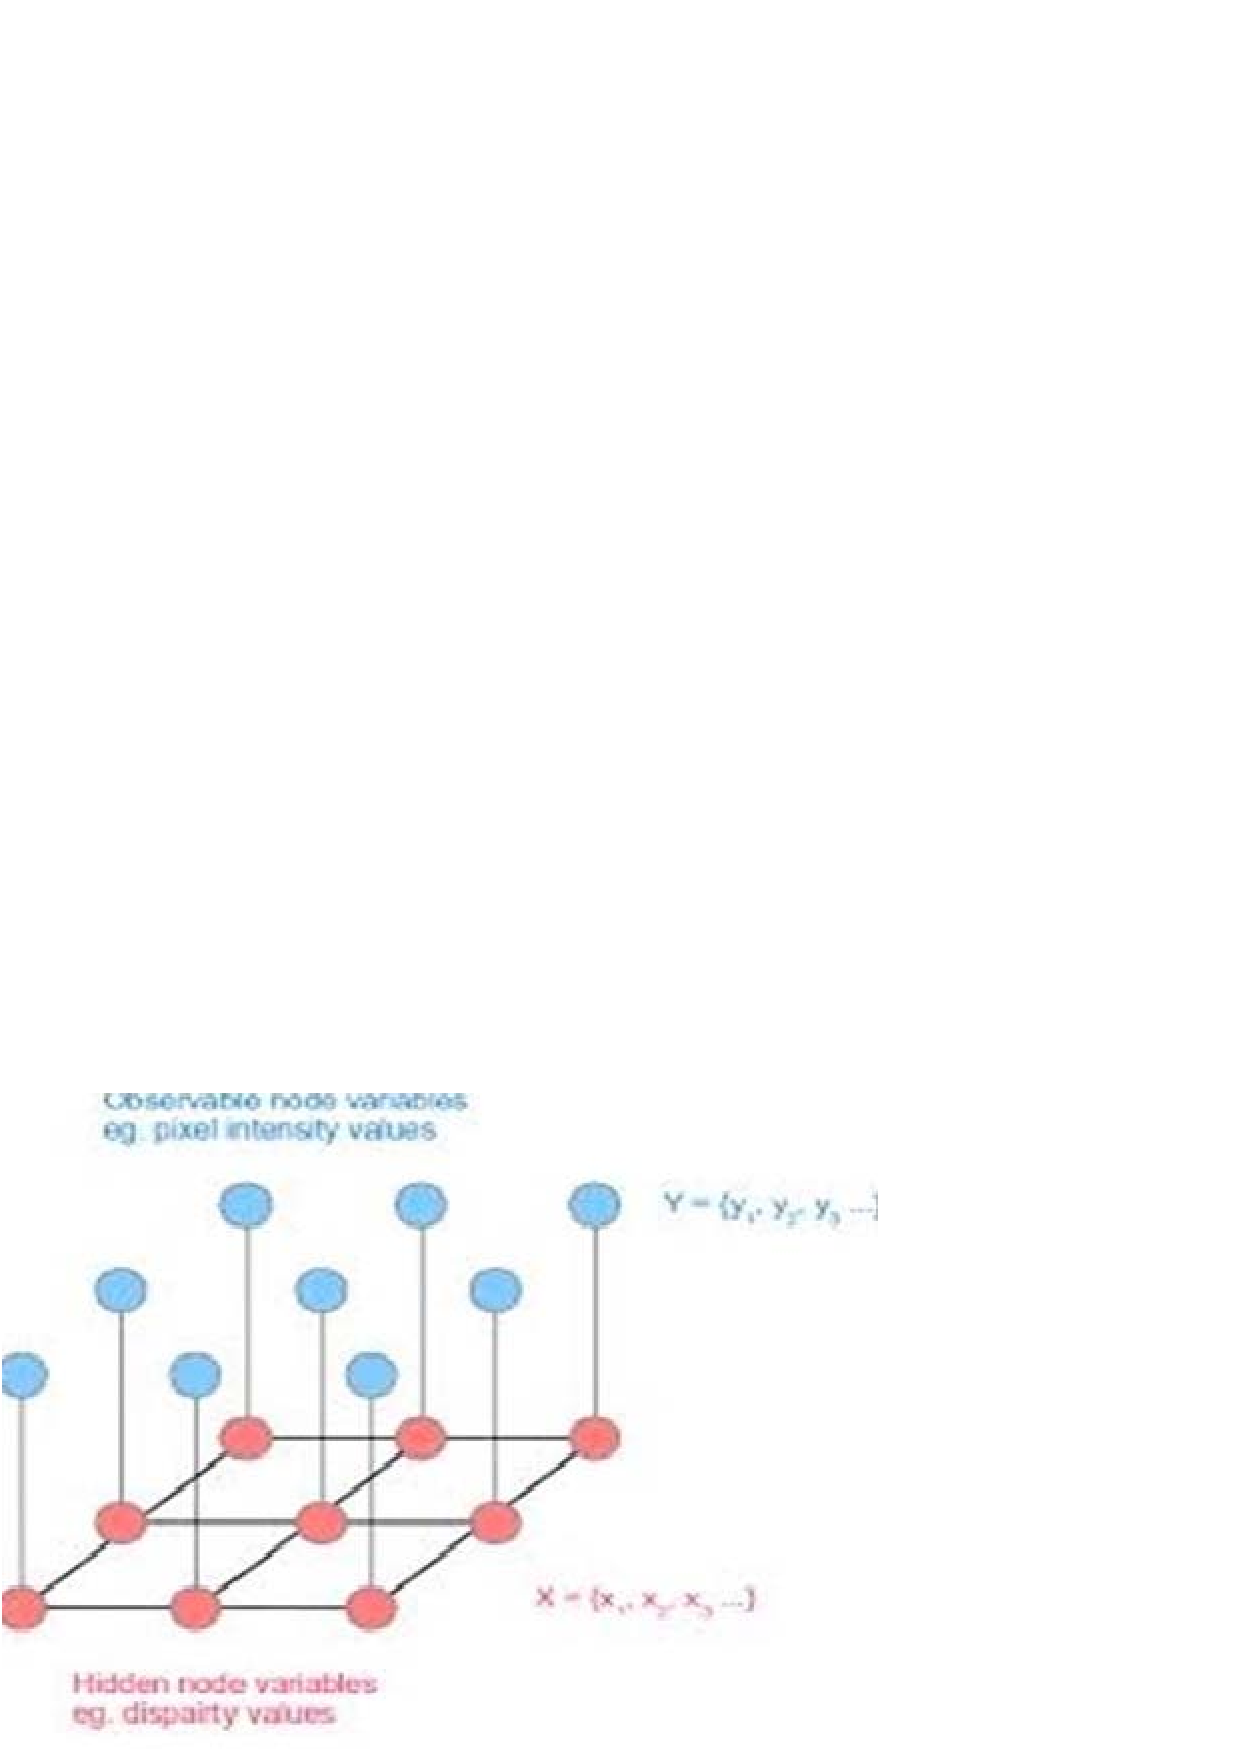
\includegraphics[width=3in]{mrf.jpg}
%\caption{MRF on 3x3 Image} \label{mrf}
%\end{center}
%\end{figure}
\end{frame}
\begin{frame}
\frametitle{Research Plan (MRF Formulation)}
\begin{itemize}
\item The  stereo problem can formulate in terms of MRF as energy functions. The energy functions basically sum up all the cost at each link for a given image and label.
\item The aim is to find label that produces lowest energy. The energy function consists of two functions, datacost function and smoothnesscost function.
\item The datacost function finds the cost ie.assigning label value to data.The function used for this is absolute difference function.
\end{itemize}
\end{frame}
\begin{frame}
\frametitle{Research Plan (MRF Formulation)}
\begin{itemize}
\item The SmoothnessCost function known as  the pairwise energy or term or potential
 \item  SmoothnessCost function  enforces smooth labeling across adjacent hidden nodes ie a function that penalizes adjacent labels that  are different
\item Some commonly used cost functions are
\begin{enumerate}
\item Binary  function
\item Linear   function
\item Quadratic function
\end{enumerate}
\end{itemize}
\end{frame}
\begin{frame}
\frametitle{Research Plan (MRF Formulation)}
commonly used Smoothnesscost functions.
%\begin{figure}[h]
%%\begin{center}
%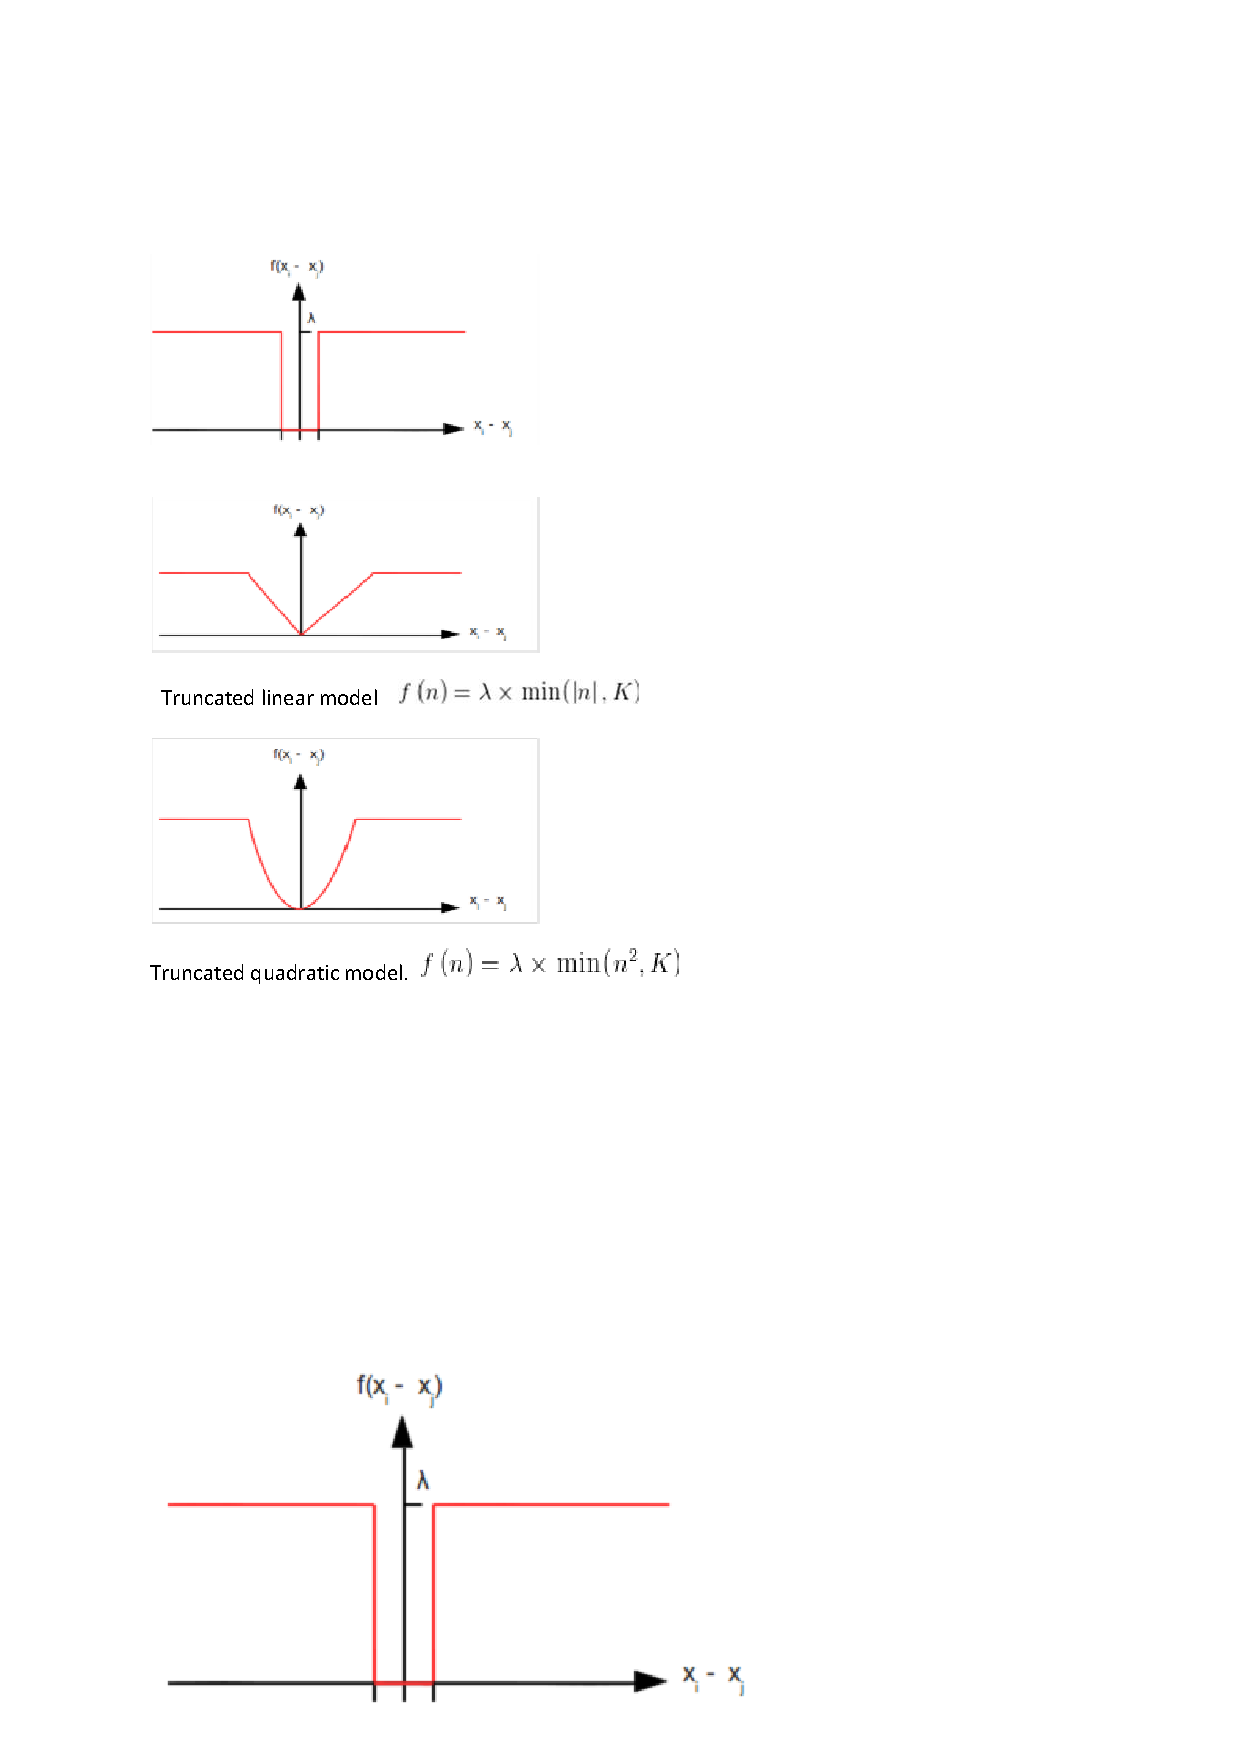
\includegraphics[width=2in]{SM.pdf}
%%\caption{MRF on 3x3 Image} \label{}
%%\end{center}
%\end{figure}
\end{frame}
\begin{frame}
\frametitle{Research Plan (MRF Formulation)}
\begin{itemize}
\item A binary function with a single tunable variable. This value controls how much smoothing is applied.
\item The linear and quadratic models have an extra parameter K. K is a truncation value that caps the maximum penalty.
\item Choosing a suitable DataCost and Smoothness function as well as the parameter is important criteria for stereo technique
\end{itemize}
\end{frame}


\begin{frame}
\frametitle{Research Plan (Application of  BP)}
\begin{itemize}


\item BP algorithm is one of the algorithm  used to find an approximate solution for an MRF.
\item  BP is message passing algorithm , A node passes a message to an adjacent node only when it is received all incoming messages, excluding the message from the destination node itself.
\end{itemize}
\end{frame}

\begin{frame}
\frametitle{Research Plan (Application of  BP)}
\%begin{figure}[h]
%\begin{center}
%Below diagram shows message passed from $x_{1}$ to$ x_{2}$
%\includegraphics[width=3in]{bp.jpg}
%\caption{Message Passage in BP} \label{mrf}
%\end{center}
%\end{figure}
\end{frame}
\begin{frame}
\frametitle{Research Plan (Application of  BP)}
\begin{itemize}
\item To  implement Belief Propagation two decisions should be made
\end{itemize}
\begin{enumerate}
\item First one is max-product algorithm is used  which finds the MAP estimate of the whole MRF
\item The second choice is Message Update Schedule
\end{enumerate}
\end{frame}
\begin{frame}
\frametitle{Research Plan (Application of BP)}
\begin{itemize}
\item An message schedule is to propagate messages in one direction and update each node immediately.
\item For instance first node is in a row ,i would send message to the node at its right,i+1.Node i+1 would then use this message immediately along with the previously received from above and below to compute the message to the node i+2.
\item Once this has been completed for every row,the same procedure occurs in the up,down and left directions. This schedule would only require one iterations for this information to propagated.
\item This feature of the $"up-down-right-left"$ message passing schedule causes the belief propagation algorithm to converge very quickly.
\end{itemize}
\end{frame}
\begin{frame}
\frametitle{Research Plan (Application of BP)}
%\begin{figure}
%%\begin{center}
%Below diagram shows Message Update Schedule in BP
%\includegraphics[width=5in]{msgsc.pdf}
%\caption{Message schedule in BP}\label{msgsc}
%%\end{center}
%\end{figure}
\end{frame}

\begin{frame}
\frametitle{Research Plan}
%\begin{figure}
%  % Requires \usepackage{graphicx}
%  \includegraphics[width=4in]{rp1.pdf}
%  \caption{Research design } \label{rp}
%\end{figure}
\end{frame}


\begin{frame}
\frametitle{The problem statement and Expected Results}
\begin{itemize}

\item By using different message passing schemes in belief propagation for stereo matching  can reduce computational time of algorithm.The execution time of belief propagation reduces after certain stability or convergence criteria met,but termination of algorithm is depend on  application of data.

\item Development of a new or modify Belief Propagation optimization method by using different message passing scheme for stereo matching applications or cases of 3D objects.\\ And  Comparative analysis of new method with existing method.\\
 \item MATLAB is used to simulate functions in the proposed  research work.
\end{itemize}
\end{frame}

\begin{frame}
\frametitle{Conclusion}
\begin{itemize}
\item The literature survey on major contributions in optimization of stereo matching technique  using Belief Propagations are studied.
  \item The operational concepts and terms related to Markov Random Field and Belief propagation are studied.
  \item The implementation of stereo matching using BP are studied and understands  the issues in implementation.
\end{itemize}
\end{frame}




\begin{frame}
\begin{enumerate}
\frametitle{bibliography}
\item  Chia-Kai Liang,Chao-Chung Cheng,Yen-Cheieh Lai, ``A Hardware-Efficient Belief Propagation'', \emph{IEEE Transactions On Circuits And Systems For Video Technology }, Vol;21,No.5,May,pp, 2011.
\item Pedro F. Felzenszwalb,Daniel P.Huttenlocher, ``A Efficient Belief Propagation For Early Vision'', \emph{International Journal Of  Computer Science  }, Vol. 41-54, No.2, February, pp, 2006.

\item Li Zhou, Tao Sun, Yuanzhi Zhan and Jia Wang, ``Software and Hardware Implementations of Stereo Matching,
'', \emph{International Journal of Electronics and Informatics}, Vol.7, No.4 (2014), pp.37-562, No.1, 2014.

\item http://nghiaho.com/notes/Markov Random Field,Loopy Belief Propagation,stereovision.
\item Tappen,M.F. and Freeman,W.T., `` Comparision of graph cuts with BP for stereo,using identical MRF parameters '', \emph{In IEEE International conference on computer vision},2003.
\end{enumerate}
\end{frame}
\begin{frame}
\begin{enumerate}
\frametitle{bibliography}
\item  Jianguo Ding,`` Probabilistic Inferences In Bayesian Networks'', \emph{International Journal Of Computer Science, Arxiv:1011.0935V2,}, 5 November 2010.
\item Frank R.Kschischang,Brendan J.Frey,Hans Andrea Loeliger, `` Factor Graph and The Sum Product Algorithm'', \emph{IEEE Transcations On Information Theory} ,Vol 47. No.2, Feb,2001.

\item Erik.B.Sudderth And William T.Freeman , ``Signal And Image Processing With Belief Propagation '', \emph{Accepted To Appear In IEEE Signal Processing Magazine}

\item  Dan Yuan, ``Understanding Belief Propagation And Its Applicatons'', \emph{Department Of Computer Engineering,University Of California}.
\item W Freeman,E.C.,Pasztor and O.T.Carmichal, `` Learning Low level Vision '', \emph{In International  journel of computer vision},40(1);25-47,2000
\end{enumerate}
\end{frame}
%Slide which includes last slides
\begin{frame}
\centerline{\textbf{\begin{Huge}Thank You...\end{Huge}}}
\end{frame}



\end{document}

